\chapter{Kiểm thử và đánh giá}
\label{chap:danh_gia}

Chương này trình bày kế hoạch kiểm thử (Mục~\ref{sec:ke-hoach-kiem-thu}), chất lượng tìm kiếm của các cấu hình (Mục~\ref{sec:danh-gia-cot-loi}) và độ trễ cùng chi phí (Mục~\ref{sec:danh-gia-dau-ra}). Tiếp theo là phân tích lỗi và đối soát nhãn (Mục~\ref{sec:phan-tich-loi}), phần trả lời các câu hỏi nghiên cứu (Mục~\ref{sec:tra-loi-ch}) và hạn chế của đánh giá (Mục~\ref{sec:han-che-danh-gia}).

\section{Kế hoạch kiểm thử}
\label{sec:ke-hoach-kiem-thu}

Kiểm thử diễn ra ở ba mức. Mức thứ nhất là kiểm thử tự động cho phần mềm, gồm 21 tệp với 222 hàm kiểm thử (đếm tĩnh; số ca thực tế nhiều hơn vì có tham số hoá). Lần chạy mặc định có 246 ca đạt, không ca nào lỗi. Có 13 ca cần GPU, cần Qdrant hoặc chạy lâu nên không nằm trong lần chạy này, và chưa rõ chúng có đạt trên phiên bản mã cuối hay không. Độ phủ mã chưa được đo.

Mức thứ hai là đánh giá chất lượng tìm kiếm trên 155 truy vấn tiếng Việt. Mức thứ ba là đo độ trễ của từng cấu hình. Bảng~\ref{tab:kt} liệt kê các hạng mục, yêu cầu phi chức năng tương ứng (Bảng~\ref{tab:c3_nfr}) và trạng thái.

\begin{table}[H]
\centering
\caption{Kế hoạch kiểm thử, yêu cầu phi chức năng tương ứng và trạng thái thực hiện}
\label{tab:kt}
\footnotesize
\renewcommand{\arraystretch}{1.05}
\begin{tabularx}{\textwidth}{@{}l >{\raggedright\arraybackslash}X l >{\raggedright\arraybackslash}p{4.6cm}@{}}
\toprule
\textbf{Mã} & \textbf{Đối tượng kiểm và cách kiểm} & \textbf{NFR} & \textbf{Kết quả} \\
\midrule
KT01 & Bộ chỉ số (Recall, MRR, nDCG, $\kappa$, bootstrap): 15 hàm kiểm thử đối chiếu giá trị tính tay & NFR04 & Đạt \\
KT02 & API web (truy vấn chữ và ảnh, ràng buộc đầu vào, khoá truy cập, lỗi kho vector): 28 hàm kiểm thử, không qua trình duyệt & NFR06, NFR07 & Đạt \\
KT03 & Lập chỉ mục, bảng đăng ký thành phần, công cụ gán nhãn, kiểm định, phân tích lỗi: 65 hàm kiểm thử & NFR03, NFR05 & Đạt \\
KT04 & Chất lượng của năm hệ chính: 155 truy vấn, nhãn của người chấm & NFR04 & Đã đo (Mục~\ref{sec:so-sanh-cau-hinh}) \\
KT05 & Ablation các trục 1, 2, 3 và 7 & -- & Đã đo bốn trục (Mục~\ref{sec:ablation}) \\
KT06 & Kiểm định thống kê: bootstrap ghép cặp, 10.000 lần lặp & -- & Đã làm (Mục~\ref{sec:kiem-dinh}) \\
KT07 & Độ trễ và chi phí: 155 truy vấn, từng truy vấn một & NFR01 & Đã đo; hệ DoRA chưa đạt chỉ tiêu 200~ms \\
KT08 & Đối soát nhãn tự động: đếm lại tệp nhãn, tính lại theo bộ lọc đã sửa & -- & Phát hiện lỗi ở bộ lọc (Mục~\ref{sec:doi-soat-nhan}) \\
\bottomrule
\end{tabularx}
\end{table}

Đối chiếu với yêu cầu phi chức năng của Chương~\ref{chap:thiet_ke}: NFR02 đến NFR07 đạt ở mức kiểm thử tự động; riêng NFR02 dựa trên lần chạy mặc định không có lỗi. NFR01 chưa đạt với hệ DoRA (Mục~\ref{sec:danh-gia-dau-ra}) và đạt với bốn hệ còn lại. NFR08 chưa đạt: catalog có 6.963 ảnh, thấp hơn ngưỡng 20.000 sản phẩm của đề cương.

\section{Đánh giá chất lượng tìm kiếm}
\label{sec:danh-gia-cot-loi}

\subsection{Dữ liệu và cách đo}
\label{sec:du-lieu-cach-do}

Catalog là tập kiểm tra gồm 6.963 ảnh Fashionpedia~\cite{jia2020fashionpedia}, chia sau khi lọc trùng và chưa từng dùng khi tinh chỉnh. Mỗi ảnh là một người mặc cả bộ: tiêu đề liệt kê trung bình 2,95 món (từ 1 đến 11 món), còn catalog chỉ lưu một danh mục chính cho mỗi ảnh. Văn bản đi kèm chỉ là tên các danh mục, không có màu, chất liệu hay mô tả của người bán.

Bộ truy vấn gồm 155 câu tiếng Việt do một người soạn, không lấy lại chú thích gốc của Fashionpedia, dài trung bình 6,62 từ, chia thành bốn nhóm. Nhóm A (46 câu) hỏi một thuộc tính, như ``áo len dệt kim xám''. Nhóm B (41 câu) hỏi nhiều thuộc tính, như ``áo len cổ tim mỏng màu than mặc mùa thu''. Nhóm C (33 câu) dùng từ địa phương hoặc từ mượn tiếng Anh, như ``giày sneaker trắng basic''. Nhóm D (35 câu) hỏi theo phong cách, như ``đồ dạo phố năng động mùa hè''.

Truy vấn được đưa vào mọi hệ nguyên văn, chỉ chuẩn hoá Unicode và chuyển về chữ thường; không dịch, không viết lại. Các hệ zero-shot (dùng nguyên mô hình đã huấn luyện sẵn) không có tham số nào chọn theo bộ này. Với hệ DoRA, nhóm chọn bản trọng số tốt nhất theo Recall@5 trên tập xác thực, dùng tên danh mục làm truy vấn giả; 155 truy vấn không tham gia việc chọn này.

Nhãn được lập theo quy trình ở Hình~\ref{fig:ch5-quytrinh}. Ở vòng 1, 10 kết quả đầu của bốn hệ đầu (BM25, CLIP, SigLIP 2 gốc, ViSigLIP-OT) được gộp thành một tập ứng viên, xáo trộn và ẩn tên hệ. Khi có hệ DoRA, vòng 2 bổ sung 10 kết quả đầu của hệ này, chỉ phần chưa có nhãn. Ba hệ ablation (LoRA thường, không mẫu âm khó, SigLIP 1) không nằm trong tập ứng viên nên một phần cặp của chúng chưa có nhãn (Mục~\ref{sec:ablation}). Mỗi cặp (truy vấn, ảnh) do hai người chấm độc lập theo thang 0 (không liên quan), 1 (liên quan một phần), 2 (liên quan chính xác). Một cặp được tính là liên quan khi điểm trung bình từ 1 trở lên; cặp hai người chấm $0$ và $2$ là liên quan, cặp $0$ và $1$ không liên quan.

Một phần cặp được tự động gán điểm 0 trước khi người chấm nhìn thấy. Vòng 1 gồm 6.079 cặp (4.011 do người chấm, 2.068 tự động); vòng 2 gồm 1.245 cặp (940 và 305). Tính chung hai vòng đầu: 7.324 cặp, trong đó 4.951 do người chấm và 2.373 tự động. Vòng 3 chỉ phục vụ ablation trục 2 và SigLIP 1: trong 1.262 cặp có 403 cặp tự động, 859 cặp còn lại không có người chấm.

Bộ lọc tự động gán điểm 0 cho cặp mà danh mục chính của ảnh không chứa từ khoá của truy vấn, để người chấm khỏi xem hàng nghìn cặp hiển nhiên sai. Với mỗi truy vấn, bộ lọc chọn danh mục đầu tiên có một từ dài hơn hai ký tự xuất hiện trong câu (khớp theo chuỗi con). Sau đó bộ lọc loại mọi ảnh mà danh mục chính không chứa từ đầu của tên danh mục đã chọn. Do mỗi ảnh chỉ lưu một danh mục chính và phép khớp theo chuỗi con quá lỏng, bộ lọc loại nhầm cả những ảnh có đúng món được hỏi. Các cặp tự động chiếm 32,4\% trong 7.324 cặp có nhãn của hai vòng đầu. Mục~\ref{sec:doi-soat-nhan} đối soát các cặp này; Mục~\ref{sec:sau-sua-loc} tính lại kết quả theo quy tắc đã sửa.

\begin{figure}[H]
\centering
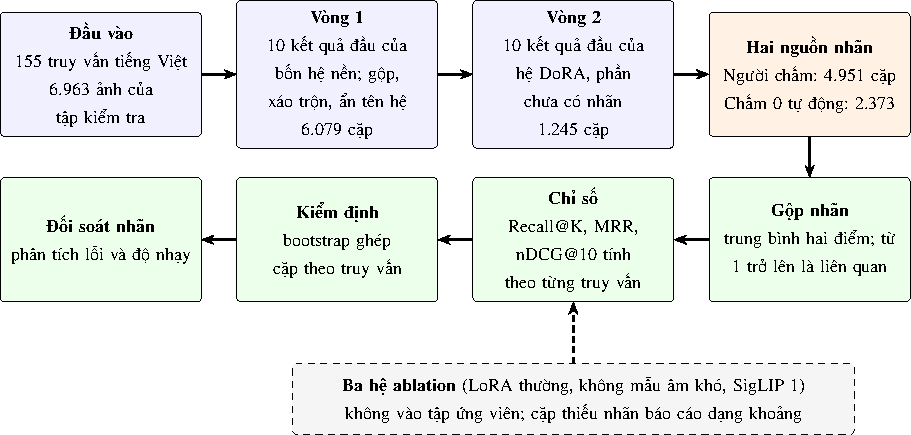
\includegraphics[width=\textwidth]{graphics/fig_ch5_1.pdf}
\caption{Quy trình đánh giá từ truy vấn đến kiểm định thống kê và đối soát nhãn}
\label{fig:ch5-quytrinh}
\end{figure}

Vòng 3 không phủ trục 1, nên trục 1 vẫn thiếu nhãn ở 102 cặp (6,6\%). Các số ở những mục sau dùng nhãn của hai vòng đầu; ô ablation dùng thêm nhãn vòng 3 và báo cáo dưới dạng khoảng (Mục~\ref{sec:ablation}).

Trong 4.951 cặp do người chấm, 4.655 cặp có hai người và 296 cặp có ba người; điểm của mỗi cặp là trung bình, người thứ ba không dùng để phân xử. Hệ số Cohen's $\kappa$ giữa từng đôi người chấm là 0,520 (3.545 cặp chung), 0,442 (1.219 cặp) và 0,441 (779 cặp). Cả ba ở mức trung bình theo thang $\kappa$ của Landis--Koch~\cite{landis1977kappa}, nên nhãn còn nhiễu, nhất là ở ranh giới giữa điểm 0 và 1.

Chỉ số gồm Recall@$K$, MRR và nDCG@10 (Mục~\ref{sec:chi-so-danh-gia}). Recall@$K$ là tỷ lệ trúng (hit rate), không phải recall của BEIR. nDCG@10 bỏ 16 truy vấn mà không ảnh nào trong tập ứng viên đạt điểm 1 trở lên. MRR xét 20 kết quả đầu nhưng chỉ 10 kết quả đầu được chấm đủ; nếu chỉ xét 10 kết quả, MRR lệch tối đa 0,0022 và thứ tự các hệ không đổi.

\subsection{So sánh các cấu hình}
\label{sec:so-sanh-cau-hinh}

Năm hệ có nhãn đầy đủ cho 10 kết quả đầu (Bảng~\ref{tab:ch1-he-thong}). BM25 chạy trên tên danh mục; CLIP, SigLIP 2 gốc và ViSigLIP-OT chạy zero-shot, riêng ViSigLIP-OT chạy trên CPU vì đầu ra bị NaN (giá trị không xác định) khi chạy trên GPU. Hệ DoRA là SigLIP 2 tinh chỉnh bằng DoRA với mẫu âm khó (Mục~\ref{sec:tinh-chinh}).

Bảng~\ref{tab:ket-qua-chinh} cho thấy cùng một thứ tự ở cả năm chỉ số: hệ DoRA, SigLIP 2 gốc, BM25, CLIP, ViSigLIP-OT. SigLIP 2 gốc có Recall@10 là 0,865, cao hơn BM25 (0,568) 29,7 điểm phần trăm, mà không cần dịch hay tinh chỉnh. Hai cột cuối là cận trên sau khi sửa bộ lọc chấm 0 tự động, với 641 cặp được tính lại (Mục~\ref{sec:sau-sua-loc}); các cột còn lại dùng nhãn hiện có. Giá trị in đậm là cao nhất mỗi cột.

\begin{table}[H]
\centering
\caption{Kết quả của năm hệ chính trên 155 truy vấn}
\label{tab:ket-qua-chinh}
\small
\renewcommand{\arraystretch}{1.12}
\setlength{\tabcolsep}{4pt}
\begin{tabular}{@{}l ccccc cc@{}}
\toprule
 & \multicolumn{5}{c}{\textbf{Nhãn hiện có}} & \multicolumn{2}{c}{\textbf{Cận trên}} \\
\cmidrule(lr){2-6}\cmidrule(lr){7-8}
\textbf{Hệ} & \textbf{R@1} & \textbf{R@5} & \textbf{R@10} & \textbf{MRR} & \textbf{nDCG@10} & \textbf{R@1} & \textbf{R@10} \\
\midrule
SigLIP 2 + DoRA & \textbf{0,697} & \textbf{0,852} & \textbf{0,884} & \textbf{0,766} & \textbf{0,684} & \textbf{0,839} & \textbf{1,000} \\
SigLIP 2 gốc & 0,490 & 0,774 & 0,865 & 0,606 & 0,449 & 0,613 & 0,987 \\
BM25 & 0,200 & 0,471 & 0,568 & 0,318 & 0,179 & 0,316 & 0,684 \\
CLIP ViT-B/32 & 0,168 & 0,381 & 0,426 & 0,252 & 0,139 & 0,206 & 0,555 \\
ViSigLIP-OT & 0,084 & 0,226 & 0,277 & 0,145 & 0,066 & 0,097 & 0,355 \\
\bottomrule
\end{tabular}
\end{table}

Tinh chỉnh tăng nhiều nhất ở các chỉ số nhạy với thứ hạng: Recall@1 tăng từ 0,490 lên 0,697 và nDCG@10 từ 0,449 lên 0,684, còn Recall@10 chỉ nhích từ 0,865 lên 0,884 (hiệu 0,019, $p = 0{,}240$; Mục~\ref{sec:kiem-dinh}). Mức tăng vì thế tập trung ở thứ hạng đầu; ở khả năng có ảnh đúng trong 10 kết quả chưa quan sát được khác biệt.

CLIP không hơn BM25 ở thứ hạng đầu, và ViSigLIP-OT thấp nhất ở mọi chỉ số. Nhóm chưa tìm ra nguyên nhân khiến ViSigLIP-OT thấp: có thể do lệch miền dữ liệu, cũng có thể do cách tích hợp mô hình chưa được đối chiếu với bản gốc. Kết luận vì vậy chỉ áp dụng cho thiết lập này.

Vị trí của BM25 và CLIP cần đọc kèm hướng lệch của nhãn. Bộ lọc và BM25 cùng dựa vào tên danh mục. Bộ lọc chỉ gán điểm 0, không bao giờ gán điểm cao, nên nó chỉ làm giảm điểm của các hệ có nhiều kết quả bị lọc. Trong 10 kết quả đầu, cặp mang nhãn tự động chiếm 20,3\% ở BM25 và 23,9\% ở hệ DoRA, còn ở SigLIP 2 gốc, CLIP và ViSigLIP-OT là 33,6\%, 39,3\% và 42,3\%. Các hệ nhìn ảnh, nhất là CLIP, vì vậy bị bất lợi hơn BM25, và việc BM25 cao hơn CLIP ở Recall@10 ($p = 0{,}003$) có thể một phần do nhãn.

Sau khi tính lại, BM25 vẫn cao hơn CLIP (Recall@10 là 0,684 so với 0,555), nhưng đó là cận trên và chưa qua người chấm. Ngược lại, SigLIP 2 gốc vượt BM25 dù nhãn không thiên về nó. Muốn đối chứng cần một tập truy vấn thứ hai có nhãn không bị bộ lọc can thiệp (Mục~\ref{sec:han-che-danh-gia}).

Theo nhóm truy vấn (Hình~\ref{fig:ch5-nhom}), nhóm D dễ nhất với mọi hệ: Recall@10 của hai hệ SigLIP 2 là 1,000 và của BM25 là 0,971. Số này đo độ rộng của truy vấn nhiều hơn khả năng hiểu phong cách, vì một câu như ``đồ đi biển thoải mái mùa hè'' có rất nhiều ảnh phù hợp. BM25 yếu nhất ở nhóm C (Recall@10 là 0,212). Hệ DoRA đạt 0,909 ở nhóm C và 0,804 ở nhóm A, nhưng khoảng tin cậy bootstrap 95\% của hai nhóm chồng nhau, nên chưa kết luận từ mượn dễ hơn từ thuần Việt.

\begin{figure}[H]
\centering
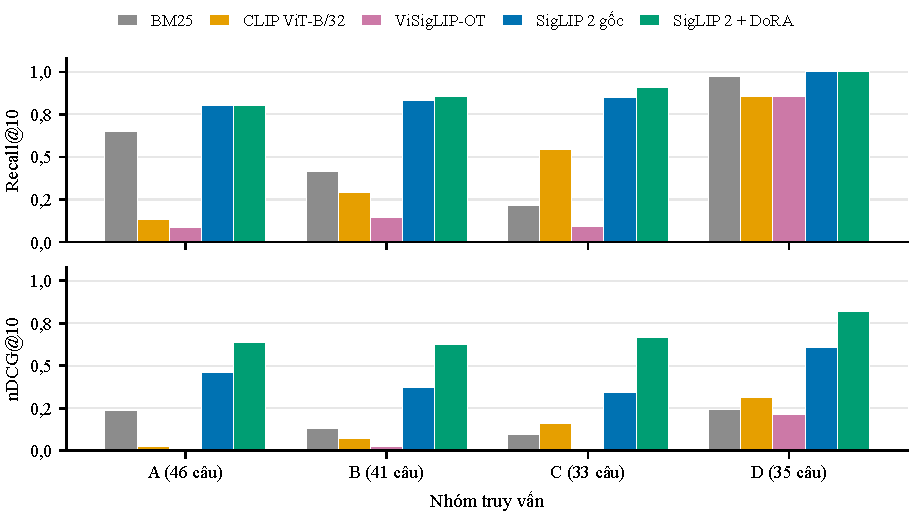
\includegraphics[width=\textwidth]{graphics/fig_ch5_3.pdf}
\caption{Recall@10 và nDCG@10 theo nhóm truy vấn}
\label{fig:ch5-nhom}
\end{figure}

\subsection{Các trục ablation}
\label{sec:ablation}

Đề cương nêu bảy trục ablation. Bốn trục đã chạy: trục 1 (DoRA so với LoRA thường), trục 2 (bật hoặc tắt mẫu âm khó), trục 3 (SigLIP 2 so với ViSigLIP-OT, xét bằng so sánh zero-shot ở Bảng~\ref{tab:ket-qua-chinh}) và trục 7 (SigLIP 1 so với SigLIP 2, chỉ suy luận). Ba trục 4, 5, 6 (hạng LoRA, kích thước lô hiệu dụng, vị trí gắn adapter) là hướng phát triển, dành cho giai đoạn sau. Mỗi cấu hình chỉ huấn luyện một lần.

Mỗi ô của Bảng~\ref{tab:ablation} chỉ đổi một yếu tố so với cấu hình tham chiếu. Vì ba hệ ablation không nằm trong tập ứng viên, một phần cặp trong 10 kết quả đầu của chúng chưa có nhãn. Các ô vì thế được báo cáo dưới dạng khoảng, dấu ``--'' nối hai cận: cận dưới coi mọi cặp chưa chấm là không liên quan, cận trên coi tất cả là liên quan. nDCG@10 không có cận trên hợp lệ nên không báo cáo cho các ô này.

\begin{table}[H]
\centering
\caption{Kết quả ablation trên 155 truy vấn}
\label{tab:ablation}
\footnotesize
\renewcommand{\arraystretch}{1.12}
\setlength{\tabcolsep}{4pt}
\begin{tabularx}{\textwidth}{@{}>{\raggedright\arraybackslash}X c c c c c@{}}
\toprule
\textbf{Cấu hình} & \textbf{R@1} & \textbf{R@5} & \textbf{R@10} & \textbf{MRR} & \textbf{Thiếu nhãn} \\
\midrule
SigLIP 2 gốc & 0,490 & 0,774 & 0,865 & 0,606 & 0\% \\
DoRA, mẫu âm khó (tham chiếu) & 0,697 & 0,852 & 0,884 & 0,766 & 0\% \\
Trục 1: LoRA thường & 0,690 & 0,832--0,839 & 0,884--0,923 & 0,760--0,771 & 6,6\% \\
Trục 2: không mẫu âm khó & 0,697 & 0,845--0,858 & 0,858--0,884 & 0,763--0,776 & 11,3\% \\
Trục 7: SigLIP 1 zero-shot & 0,316--0,645 & 0,548--0,826 & 0,710--0,890 & 0,427--0,738 & 44,5\% \\
\bottomrule
\end{tabularx}
\end{table}

Với trục 1, LoRA thường và DoRA chưa quan sát được khác biệt ở Recall@1 ($p = 0{,}82$) và MRR ($p = 0{,}41$). Recall@10 của LoRA thường chỉ là cận dưới 0,884 và có thể tới 0,923 vì 6,6\% cặp thiếu nhãn; giá trị $p = 1{,}00$ ở Recall@10 chỉ đúng cho cận dưới. Hai hệ trùng 92\% top-10 và hiệu Recall@1 chỉ 0,0065 (một truy vấn), nên với 155 truy vấn và một lần huấn luyện cho mỗi cấu hình thì chưa có bằng chứng DoRA hơn LoRA thường.

LoRA thường huấn luyện ít tham số hơn một chút (0,31\% so với 0,33\% mô hình) và mất 7.437,6 s so với 11.084,7 s, ngắn hơn 32,9\%. Với trục 2, Recall@1 giống hệt tham chiếu ($p = 1{,}00$; ở $K = 1$ không cặp nào thiếu nhãn) và MRR chưa quan sát được khác biệt ($p = 0{,}74$). Recall@10 thấp hơn (cận dưới 0,858 so với 0,884, $p = 0{,}037$), nhưng ô này thiếu 11,3\% nhãn và cận trên của nó bằng giá trị tham chiếu, nên chưa kết luận được. Bước đào mẫu âm khó làm huấn luyện lâu hơn 28,3\% (11.084,7 s so với 8.642,1 s).

Với trục 7, khoảng Recall@1 của SigLIP 1 ($[0{,}316;\,0{,}645]$) chứa giá trị của SigLIP 2 gốc (0,490) nhưng không chứa giá trị của hệ DoRA (0,697). Vì vậy SigLIP 1 thấp hơn hệ DoRA ở Recall@1; so với SigLIP 2 gốc thì chưa kết luận được. Ngoài ra ảnh đầu vào của SigLIP 1 là 256 pixel thay vì 224. Với trục 3, SigLIP 2 vượt ViSigLIP-OT (Recall@1 là 0,490 so với 0,084); chưa tách được phần do mô hình và phần do cách tích hợp.

\subsection{Kiểm định thống kê}
\label{sec:kiem-dinh}

Kiểm định dùng bootstrap ghép cặp theo truy vấn~\cite{efron1993bootstrap}: chọn lại 155 truy vấn có hoàn lại, 10.000 lần, seed 42, hai phía, mức $0{,}05$. Cách này thay cho McNemar vì MRR không phải chỉ số nhị phân và cả năm hệ chạy trên cùng 155 truy vấn. Giá trị $p$ ghi bằng $0$ trong tệp kết quả được viết là $p < 10^{-4}$, đúng độ phân giải của 10.000 lần lặp. SigLIP 1 bị loại khỏi kiểm định vì lúc chạy (trước vòng 3), 67\% cặp trong 10 kết quả đầu của nó chưa có nhãn. Giá trị $p$ so với nó khi đó phản ánh việc thiếu nhãn hơn là chất lượng của hệ. Kết quả nằm ở Bảng~\ref{tab:kiem-dinh}.

\begin{table}[H]
\centering
\caption{Kiểm định bootstrap ghép cặp trên 155 truy vấn}
\label{tab:kiem-dinh}
\small
\setlength{\tabcolsep}{4pt}
\renewcommand{\arraystretch}{1.12}
\begin{tabular}{@{}l r r r r r r@{}}
\toprule
 & \multicolumn{2}{c}{\textbf{Recall@1}} & \multicolumn{2}{c}{\textbf{Recall@10}} & \multicolumn{2}{c}{\textbf{MRR}} \\
\cmidrule(lr){2-3}\cmidrule(lr){4-5}\cmidrule(lr){6-7}
\textbf{So sánh} & $\Delta$ & $p$ & $\Delta$ & $p$ & $\Delta$ & $p$ \\
\midrule
DoRA $-$ SigLIP 2 gốc & $+0{,}206$ & $<10^{-4}$ & $+0{,}019$ & $0{,}240$ & $+0{,}160$ & $<10^{-4}$ \\
SigLIP 2 gốc $-$ BM25 & $+0{,}290$ & $<10^{-4}$ & $+0{,}297$ & $<10^{-4}$ & $+0{,}289$ & $<10^{-4}$ \\
SigLIP 2 gốc $-$ CLIP & $+0{,}323$ & $<10^{-4}$ & $+0{,}439$ & $<10^{-4}$ & $+0{,}355$ & $<10^{-4}$ \\
BM25 $-$ CLIP & $+0{,}032$ & $0{,}481$ & $+0{,}142$ & $0{,}003$ & $+0{,}066$ & $0{,}070$ \\
BM25 $-$ ViSigLIP-OT & $+0{,}116$ & $0{,}001$ & $+0{,}290$ & $<10^{-4}$ & $+0{,}173$ & $<10^{-4}$ \\
CLIP $-$ ViSigLIP-OT & $+0{,}084$ & $0{,}015$ & $+0{,}148$ & $0{,}002$ & $+0{,}107$ & $0{,}001$ \\
\bottomrule
\end{tabular}
\end{table}

Trong Bảng~\ref{tab:kiem-dinh}, $\Delta$ là hiệu của hệ thứ nhất trừ hệ thứ hai. Hệ DoRA tốt hơn SigLIP 2 gốc ở Recall@1 và MRR nhưng chưa quan sát được khác biệt ở Recall@10. SigLIP 2 gốc tốt hơn BM25 và CLIP ở cả ba chỉ số. ViSigLIP-OT thấp hơn cả BM25 và CLIP. BM25 và CLIP chưa phân biệt được ở Recall@1 và MRR. Bảng gồm 18 giá trị $p$ chưa hiệu chỉnh; theo ngưỡng Bonferroni $0{,}05/18 \approx 0{,}0028$, hai giá trị $0{,}003$ (BM25 so với CLIP ở Recall@10) và $0{,}015$ (CLIP so với ViSigLIP-OT ở Recall@1) chỉ là gợi ý.

\section{Độ trễ và chi phí}
\label{sec:danh-gia-dau-ra}

Độ trễ đo trên máy phát triển (GPU Quadro T2000 4~GB), với kho vector trong bộ nhớ, trên catalog 6.963 ảnh, từng truy vấn chữ một, lấy 20 kết quả đầu, bỏ 5 truy vấn khởi động. Mỗi truy vấn được đo ba thành phần: mã hoá truy vấn, tìm trong chỉ mục và tổng đầu-cuối. Chỉ tiêu của đề cương là dưới 200~ms cho một truy vấn trên một GPU. Đề cương tính cho GPU mạnh hơn máy đo, nên kết quả chỉ phản ánh máy này. Kết quả nằm ở Bảng~\ref{tab:do-tre}.

\begin{table}[H]
\centering
\caption{Độ trễ theo thành phần, p50 / p95 (ms)}
\label{tab:do-tre}
\small
\renewcommand{\arraystretch}{1.12}
\begin{tabular}{@{}l c c c c@{}}
\toprule
\textbf{Hệ} & \textbf{Thiết bị} & \textbf{Mã hoá truy vấn} & \textbf{Tìm trong chỉ mục} & \textbf{Đầu-cuối} \\
\midrule
BM25 & CPU & 0,01 / 0,03 & 8,68 / 15,69 & 14,67 / 24,13 \\
CLIP ViT-B/32 & GPU & 40,83 / 69,30 & 26,37 / 43,63 & 66,78 / 111,96 \\
SigLIP 2 gốc & GPU & 48,94 / 73,19 & 41,24 / 54,96 & 91,55 / 127,37 \\
ViSigLIP-OT & CPU & 71,38 / 87,80 & 48,12 / 56,88 & 118,25 / 146,45 \\
SigLIP 2 + DoRA & GPU & 193,59 / 663,59 & 48,61 / 127,51 & 245,57 / 746,32 \\
\bottomrule
\end{tabular}
\end{table}

Bảng~\ref{tab:do-tre} cho thấy bốn hệ đầu bảng đạt chỉ tiêu cả ở p50 lẫn p95. ViSigLIP-OT chậm nhất nhóm này (p95 là 146,45~ms) nhưng chạy trên CPU nên không so trực tiếp với các hàng GPU. Hệ DoRA không đạt: p50 là 245,57~ms và p95 là 746,32~ms. Thành phần chi phối là mã hoá truy vấn, với p50 là 193,59~ms (khoảng 4 lần SigLIP 2 gốc) và p95 là 663,59~ms (khoảng 9 lần). Adapter được nạp riêng chứ chưa gộp vào trọng số; nhóm chưa thử gộp nên chưa biết cách này có giảm được độ trễ hay không.

Lần huấn luyện tham chiếu của hệ DoRA (10 epoch trên 32.491 ảnh, lô hiệu dụng 256) mất 11.084,7 s, tức 3,08 giờ.

\section{Phân tích lỗi}
\label{sec:phan-tich-loi}

\subsection{Đối soát bộ lọc chấm 0}
\label{sec:doi-soat-nhan}

Cách bộ lọc hoạt động đã nêu ở Mục~\ref{sec:du-lieu-cach-do}. Đối soát đánh dấu 35 truy vấn bị bộ lọc ảnh hưởng, chia thành ba nhóm rời nhau.

\textbf{Phụ kiện (14 truy vấn, 406 cặp).} Ảnh người đeo kính, xách túi hay đi giày có danh mục chính là một món áo hoặc váy. Vì vậy chúng nhận điểm 0 ở các truy vấn kính, băng đô, cà vạt, đồng hồ, dây nịt, giày, túi và khăn choàng, dù tiêu đề ảnh có món được hỏi.

\textbf{Từ khoá giả (12 truy vấn, 393 cặp).} Bộ lọc khớp một từ ngắn nằm trong cụm khác và lấy nhầm danh mục. Từ ``dài'' trong ``tay dài'' kéo theo ``Quần dài''; từ ``tay'' trong ``găng tay'' kéo theo ``Áo choàng không tay''; từ ``váy'' trong ``váy hai dây'' kéo theo ``Chân váy''.

\textbf{Từ khoá đầm (9 truy vấn, 131 cặp).} Truy vấn viết ``đầm'' còn tên danh mục là ``Váy đầm'', nên từ đầu ``váy'' không có trong câu và truy vấn bị đánh dấu. Ở nhóm này bộ lọc chọn đúng loại sản phẩm. Nhóm này vẫn được giữ trong 35 truy vấn vì quy tắc đánh dấu chạy tự động, không để người viết quyết định truy vấn nào ở lại.

Như vậy bộ lọc gán nhãn sai ở 26 truy vấn (14 phụ kiện và 12 từ khoá giả; 799 cặp). Cả 18 truy vấn mà hệ DoRA trượt Recall@10 đều nằm trong 26 truy vấn này: 14 phụ kiện và 4 từ khoá giả (41, 57, 64, 148), không truy vấn nào thuộc nhóm đầm. SigLIP 2 gốc trượt 21 truy vấn, trong đó 19 nằm trong 35 truy vấn bị đánh dấu.

Người chấm có xem ảnh cả bộ ở 10 truy vấn phụ kiện (mã 15, 18, 22, 25, 26, 35, 40, 73, 75, 101; mũ, vớ, dù, ví, găng tay, khăn). Ở 6 trong số đó (18, 25, 35, 40, 73, 75) người chấm chỉ thấy các cặp đã lọt qua bộ lọc; 4 truy vấn còn lại (15, 22, 26, 101) không bị bộ lọc ảnh hưởng. Trong các cặp do người chấm xem, 82 trên 138 cặp (59,4\%) có món được hỏi trong tiêu đề được chấm liên quan, so với 6 trên 169 cặp (3,6\%) khi ảnh không có món đó. Mẫu này nghiêng về các món dễ thấy, nên tỷ lệ chỉ cho biết người chấm có thể chấp nhận ảnh cả bộ.

\subsection{Các truy vấn lỗi nặng nhất}
\label{sec:hai-muoi-loi}

Phân tích lấy hệ DoRA làm đối tượng, SigLIP 2 gốc làm mốc, $K = 10$, trên 20 truy vấn. Đó là 18 truy vấn mà hệ DoRA không có ảnh liên quan trong 10 kết quả đầu, cộng hai truy vấn mà hệ DoRA kém SigLIP 2 gốc nhiều nhất. Xem lại nguồn gốc các nhãn 0 cho thấy phần lớn do bộ lọc chứ không do người chấm: 16 trong 20 truy vấn có cả 10 kết quả đầu mang nhãn 0 tự động. Vì vậy nhóm không dùng các nguyên nhân gán bằng tay, như ``ảnh chứa nhiều sản phẩm'', làm kết luận. Ở ``áo sơ mi lụa tay dài công sở màu trắng ngà'' (41), bộ lọc khớp từ ``dài'' với danh mục ``Quần dài'' nên gán điểm 0 cho mọi ảnh không có quần dài. Ở ``giày cao gót đen'' (23), ảnh đứng đầu có danh mục chính là đầm nên nhận điểm 0 dù người mẫu đi giày.

\subsection{Kết quả sau khi sửa bộ lọc}
\label{sec:sau-sua-loc}

Vì chưa thể chấm lại toàn bộ các cặp bị lọc, nhóm tính lại theo một quy tắc đã sửa. Với 35 truy vấn bị đánh dấu, nhóm gán thủ công danh mục được hỏi sau khi đã xem các ca lỗi. Một cặp bị chấm 0 tự động được tính là liên quan nếu danh mục đó có trong tiêu đề ảnh, kể cả khi không phải danh mục chính. Có 641 cặp được tính lại (398 ở truy vấn phụ kiện, 238 ở từ khoá giả, 5 ở từ khoá đầm); các cặp còn lại giữ nhãn cũ.

Hai cột cuối của Bảng~\ref{tab:ket-qua-chinh} là kết quả tính lại. Đó là cận trên chứ không phải số đo: quy tắc coi mọi ảnh chứa món được hỏi là liên quan, trong khi người chấm chỉ chấp nhận 59,4\% số đó ở các truy vấn phụ kiện đã chấm. Thứ tự năm hệ không đổi ở cả hai chỉ số. Bootstrap với nhãn đã sửa cho cùng kết luận về hai hệ đầu bảng: hệ DoRA tốt hơn ở Recall@1 ($+0{,}226$, $p < 10^{-4}$) và chưa quan sát được khác biệt ở Recall@10 ($+0{,}013$, $p = 0{,}272$).

Mức lỗi do nhãn chưa định lượng được. Mỗi truy vấn trong 18 truy vấn trượt có từ 3 đến 10 ảnh chứa món được hỏi nhưng bị chấm 0 tự động ở 10 kết quả đầu. Nếu người chấm chấp nhận mọi ảnh đó, cả 18 truy vấn đều có ảnh liên quan. Nếu chỉ chấp nhận 59,4\% như ở các truy vấn phụ kiện đã chấm, số truy vấn có ảnh đúng nằm trong khoảng 11 đến 18, tuỳ mức độ các ảnh của cùng một truy vấn được chấp nhận cùng nhau. Riêng tỷ lệ 59,4\% dao động từ 0,33 đến 1,00 giữa các truy vấn.

Bảng chính là kết quả trên cả 155 truy vấn. Nhóm bỏ 35 truy vấn do bộ lọc đánh dấu để làm phân tích độ nhạy. Tập này được chọn sau khi đã xem các ca lỗi, nên không thay thế bảng chính và không phải kết quả của hệ thống. Trên 120 truy vấn còn lại, hệ DoRA đạt Recall@1 là 0,825 và Recall@10 là 1,000; SigLIP 2 gốc đạt 0,542 và 0,983. Nếu chỉ bỏ 26 truy vấn bị lọc sai (còn 129 truy vấn), Recall@1 là 0,822 với hệ DoRA và 0,558 với SigLIP 2 gốc. Giữ hay bỏ 9 truy vấn đầm vì vậy không đổi kết luận.

Tập 120 cũng chưa phải tập sạch: 60 truy vấn trong đó còn 1.187 cặp chấm 0 tự động, và 322 cặp ở 57 truy vấn có nguyên tên danh mục nằm trong tiêu đề ảnh dù danh mục chính khác. Đó là cận trên số cặp có thể bị gán điểm 0 oan, chưa phải số lỗi đã xác nhận.

Có hai điều không đổi. Thứ nhất, catalog thiếu ảnh phụ kiện đứng riêng: không ảnh nào trong tập kiểm tra lấy giày, túi, kính mắt, đồng hồ hay dây nịt làm danh mục chính. Thứ hai, lỗi của mô hình ở thứ hạng đầu chưa tách được khỏi lỗi nhãn: ngay với cận trên vẫn còn 25 truy vấn (16,1\%) chưa có ảnh đúng ở vị trí đầu.

\section{Trả lời các câu hỏi nghiên cứu}
\label{sec:tra-loi-ch}

\textbf{CH1. Tìm kiếm bằng biểu diễn chung đa mô thức dùng zero-shot (SigLIP~2, CLIP, ViSigLIP-OT) có tốt hơn BM25 trên truy vấn tiếng Việt không?} Có với SigLIP 2, không với CLIP và ViSigLIP-OT. SigLIP 2 gốc đạt Recall@1 là 0,490 so với 0,200 của BM25 và Recall@10 là 0,865 so với 0,568 ($p < 10^{-4}$ ở mọi chỉ số). CLIP không phân biệt được với BM25 ở Recall@1 ($p = 0{,}481$) và có xu hướng thấp hơn ở Recall@10 ($p = 0{,}003$, chưa vượt ngưỡng Bonferroni); ViSigLIP-OT thấp hơn BM25. Phạm vi của kết luận nêu ở Mục~\ref{sec:han-che-danh-gia}.

\textbf{CH2. Tinh chỉnh SigLIP~2 bằng adapter có tốt hơn zero-shot không, và DoRA hay mẫu âm khó có tốt hơn LoRA thường không?} Tinh chỉnh adapter cải thiện thứ hạng đầu, nhưng chưa tách được phần đóng góp riêng của DoRA hay của mẫu âm khó. Recall@1 tăng từ 0,490 lên 0,697 và MRR từ 0,606 lên 0,766 ($p < 10^{-4}$), còn Recall@10 tăng từ 0,865 lên 0,884 ($p = 0{,}240$).

Về ablation, LoRA thường đạt Recall@1 là 0,690 và MRR là 0,760, chưa khác DoRA ($p = 0{,}82$ và $0{,}41$), và huấn luyện nhanh hơn 32,9\%; Recall@10 của nó nằm trong khoảng 0,884 đến 0,923 (Mục~\ref{sec:ablation}). Bản tắt mẫu âm khó có Recall@1 bằng bản tham chiếu và MRR nằm trong khoảng 0,763 đến 0,776 (tham chiếu là 0,766); Recall@10 của bản này chưa kết luận được vì thiếu 11,3\% nhãn.

Chi phí của hệ DoRA gồm 3,08 giờ huấn luyện và độ trễ p50 là 245,57~ms, chưa đạt chỉ tiêu 200~ms. Chú thích ảnh khi huấn luyện chỉ gồm tên danh mục và tên chi tiết bộ phận, không có màu hay chất liệu. Mức tăng vì thế có lẽ đến từ việc căn chỉnh tên danh mục tiếng Việt với ảnh; nhóm chưa có thí nghiệm đối chứng để xác nhận.

\textbf{CH3. Nguyên nhân lỗi còn lại nằm ở mô hình hay ở nhãn và catalog?} Với bằng chứng hiện có, phần lớn thất bại ở Recall@10 đến từ nhãn và catalog: toàn bộ 18 truy vấn trượt đều thuộc nhóm bị bộ lọc chấm 0 sai (Mục~\ref{sec:doi-soat-nhan}). Điều này chưa chứng minh mô hình không lỗi, vì ở Recall@1 vẫn còn 21 trên 120 truy vấn không bị đánh dấu mà ảnh đúng không đứng đầu, và 322 cặp bị chấm 0 có thể chấm oan. Tách hai nguyên nhân cần chấm lại các cặp này (Mục~\ref{sec:sau-sua-loc}).

\section{Hạn chế của đánh giá}
\label{sec:han-che-danh-gia}

\begin{itemize}
    \item \textbf{Bộ truy vấn:} 155 câu do một người soạn, chưa tách tập phát triển và tập giữ lại, chưa thử với người dùng thật, không có câu nào về trang phục truyền thống Việt Nam (áo dài, áo bà ba, nón lá) và toàn bộ là chữ. Đồ án đánh giá truy vấn bằng văn bản; tìm bằng ảnh và độ lệch văn hoá nằm ngoài phạm vi đánh giá. Hướng phát triển là một tập truy vấn thứ hai do người khác soạn, làm tập giữ lại.
    \item \textbf{Nhãn:} người chấm đồng thuận ở mức trung bình ($\kappa$ từ 0,44 đến 0,52), chưa có bước phân xử bất đồng, và nhãn chỉ phủ 10 kết quả đầu của tập ứng viên do năm hệ này tạo ra. Các cặp bị chấm 0 tự động chỉ được tính lại bằng quy tắc, chưa qua người chấm (Mục~\ref{sec:sau-sua-loc}), và bộ lọc lệch về phía BM25 so với các hệ nhìn ảnh (Mục~\ref{sec:so-sanh-cau-hinh}). Hướng phát triển là chấm lại các cặp này, kết hợp với tập truy vấn thứ hai nêu trên.
    \item \textbf{So sánh giữa các hệ:} mỗi cấu hình huấn luyện một lần với seed 42, nên chênh lệch nhỏ giữa các cấu hình tinh chỉnh chưa tách được khỏi phương sai giữa các lần huấn luyện. Chưa có thí nghiệm đối chứng tách việc căn chỉnh tên danh mục khỏi việc học màu và chất liệu. BM25 chỉ chạy trên tên danh mục, văn bản duy nhất của catalog. ResNet-50 kết hợp KNN, so sánh với SigLIP 2 kèm dịch máy và Qwen3-VL-Embedding nằm ngoài phạm vi đánh giá và là hướng phát triển.
    \item \textbf{Dữ liệu và phép đo:} catalog là ảnh người mặc cả bộ, không có giá hay mô tả của người bán, nên chưa suy rộng được sang sàn thương mại điện tử. Độ trễ đo trên một máy với kho trong bộ nhớ, thiết bị khác nhau giữa các hệ; độ trễ qua Qdrant và API web nằm ngoài phạm vi đánh giá. Kiểm định chưa hiệu chỉnh cho nhiều phép so sánh và chỉ xét nhiễu do lấy mẫu truy vấn.
\end{itemize}
